\documentclass[tikz,border=2pt]{standalone}
\usepackage{amsmath}
\usepackage{xcolor}

\definecolor{journalink}{HTML}{1F1C18}
\definecolor{journalmuted}{HTML}{8A7F72}
\definecolor{journalaccent}{HTML}{9C2D2D}

\begin{document}
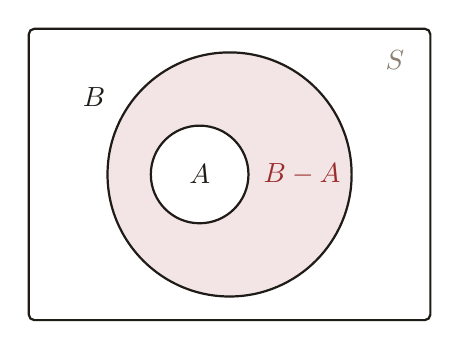
\begin{tikzpicture}[
  x=1cm,
  y=1cm,
  every node/.style={font=\normalsize}
]
  \path[
    fill=journalaccent,
    fill opacity=0.12,
    even odd rule
  ]
    (0,0) circle (1.55)
    (-0.38,0) circle (0.62);

  \draw[journalink, line width=0.8pt, rounded corners=2pt]
    (-2.55,-1.85) rectangle (2.55,1.85);
  \draw[journalink, line width=0.8pt]
    (0,0) circle (1.55);
  \draw[journalink, line width=0.8pt]
    (-0.38,0) circle (0.62);

  \node[journalink] at (-0.38,0) {$A$};
  \node[journalaccent] at (0.92,0) {$B-A$};
  \node[journalink] at (-1.72,0.98) {$B$};
  \node[journalmuted] at (2.1,1.45) {$S$};
\end{tikzpicture}
\end{document}
